\documentclass[pdflatex,en,11pt]{aghdpl}
\usepackage[english]{babel}
\usepackage{polski}
\usepackage[utf8]{inputenc}

\usepackage[backend=bibtex,
style=numeric,
sorting=none,
%bibencoding=ascii,
%style=reading,
giveninits=true
]{biblatex}
\renewbibmacro{in:}{%
    \ifentrytype{article}{}{\printtext{\bibstring{in}\intitlepunct}}}

\addbibresource{bibliografia.bib}

\DeclareNameAlias{sortname}{last-first}
\DeclareNameAlias{default}{last-first}

% dodatkowe pakiety
\usepackage{enumerate}
\usepackage{listings}
\usepackage{float}
\usepackage{siunitx}
\usepackage{hyperref}
\usepackage[acronym,nomain,toc]{glossaries}
\usepackage{graphicx}
\usepackage{enumitem}
\usepackage{multirow,bigdelim}
\usepackage{makecell}
\usepackage{subcaption}
\usepackage{multicol}
\usepackage{lipsum}
\usepackage[table]{xcolor}

% \lstloadlanguages{TeX}

\lstset{
  literate={ą}{{\k{a}}}1
           {ć}{{\'c}}1
           {ę}{{\k{e}}}1
           {ó}{{\'o}}1
           {ń}{{\'n}}1
           {ł}{{\l{}}}1
           {ś}{{\'s}}1
           {ź}{{\'z}}1
           {ż}{{\.z}}1
           {Ą}{{\k{A}}}1
           {Ć}{{\'C}}1
           {Ę}{{\k{E}}}1
           {Ó}{{\'O}}1
           {Ń}{{\'N}}1
           {Ł}{{\L{}}}1
           {Ś}{{\'S}}1
           {Ź}{{\'Z}}1
           {Ż}{{\.Z}}1
}

\usepackage{array}
\newcolumntype{L}[1]{>{\raggedright\let\newline\\\arraybackslash\hspace{0pt}}m{#1}}
\newcolumntype{C}[1]{>{\centering\let\newline\\\arraybackslash\hspace{0pt}}m{#1}}
\newcolumntype{R}[1]{>{\raggedleft\let\newline\\\arraybackslash\hspace{0pt}}m{#1}}

\makeatletter
\let\ps@plain\ps@fancy
\makeatother

%---------------------------------------------------------------------------

\author{Piotr Rzeszut}
\shortauthor{P. Rzeszut}

\course{Elektronika i Telekomunikacja}

\titlePL{Magnetyczne złącza tunelowe z anizotropią prostopadłą do zastosowań w szeregowo-równoległych połączeniach elementarnych komórek pamięci stt-mram - streszczenie}
\titleEN{Magnetic tunnel junctions with perpendicular anisotropy for use in serial and parallel connections of elementary stt-mram cells}

\shorttitlePL{Magnetyczne złącza tunelowe z anizotropią prostopadłą do zastosowań w szeregowo-równoległych połączeniach elementarnych komórek pamięci STT-MRAM} % skrócona wersja tytułu jeśli jest bardzo długi
\shorttitleEN{Magnetic tunnel junctions with perpendicular anisotropy for use in serial and parallel connections...}

\thesistypePL{Praca dyplomowa magisterska}
\thesistypeEN{Master Thesis}

\supervisorPL{dr inż. Witold Skowroński}
\supervisorEN{Witold Skowroński Ph.D}

\date{2018}

\departmentPL{Katedra Elektroniki}
\departmentEN{Department of Electronics}

\facultyPL{Wydział Informatyki, Elektroniki i Telekomunikacji}
\facultyEN{Faculty of Computer Science, Electronics and Telecommunications}

\acknowledgements{}

\setlength{\cftsecnumwidth}{10mm}

\DeclareSIUnit\rpm{rpm}

\definecolor{capping}{rgb}{0.45,0.7,0.29}
\definecolor{ferromagnetic}{rgb}{0.25,0.44,0.79}
\definecolor{barrier}{rgb}{0.65,0.65,0.65}
\definecolor{bottom}{rgb}{0.98,0.76,0}
\definecolor{substrate}{rgb}{0.42,0.64,0.86}

\newcommand\varpm{\mathbin{\vcenter{\hbox{%
  \oalign{\hfil$\scriptstyle+$\hfil\cr
          \noalign{\kern-.3ex}
          $\scriptscriptstyle({-})$\cr}%
}}}}
\newcommand\varmp{\mathbin{\vcenter{\hbox{%
  \oalign{\hfil$\scriptstyle-$\hfil\cr
          \noalign{\kern-.3ex}
          $\scriptscriptstyle({+})$\cr}%
}}}}

%---------------------------------------------------------------------------

\begin{document}

\titlepages

%\textbf{\huge CONFIDENTIAL}

    Contents of this work are the subject of patent application and proceedings. Copying, publishing or sharing of any information presented in the work is strictly prohibited until acceptance of the patent application by the patent office.

\vskip 3cm 
\textbf{\huge POUFNE}

    Zawartość niniejszej pracy jest przedmiotem wniosku i postępowania patentowego. Kopiowanie, publikowanie lub rozpowszechnianie jakichkolwiek informacji przedstawianych w tej pracy jest surowo wzbroniona do momentu przyjęcia wniosku patentowego przez urząd patentowy.
%\begin{center}
    \thispagestyle{empty}
    \vspace*{\fill}
    Rodzicom
    \vspace*{\fill}
\end{center}
%\tableofcontents

\chapter{Wstęp}
	Pamięci komputerowe dzielą się na nieulotne i ulotne. Pierwsze z nich mogą przechowywać dane bez konieczności zasilania przez długi okres czasu, ale są względnie wolne, biorąc pod uwagę czas zapisu i odczytu. Pamięci takie posiadają zwykle dużą gęstość zapisu, co uzasadnia ich stosowanie do przechowywania danych.
	
	Pamięci ulotne z kolei potrzebują stałego zasilania w celu przechowywania danych, jednak w zamian oferują bardzo szybki zapis i odczyt danych. Gęstość zapisu w takich pamięciach jest jednak mniejsza niż w wypadku nieulotnych.

	W ostatnich latach zaprezentowane zostały nowe typy pamięci \cite{fujisaki2013review,kent2015new}, które łączą zalety obu przedstawionych powyżej typów, oferując czasy zapisu-odczytu porównywalne z pamięciami ulotnymi, jednocześnie umożliwiając przechowywanie danych po odłączeniu zasilania. Obecnie najszerzej znane typy takich pamięci to FRAM, PCRAM, ReRAM oraz MRAM, których to dotyczy niniejsza praca.
    
    Pamięci MRAM, czyli magnetyczne pamięci RAM, mają praktycznie nieograniczoną ilość cykli zapisu-odczytu, a czasy dostępu moga być porównywane z pamięciami DRAM. Są dodatkowo odporne na promieniowanie jonizujące/kosmiczne. Czyni to je szczególnie interesującymi magaznyami danych do zastosowania w sondach kosmicznych, lotnictwie i innych dziedzinach, wymagających wysokiej niezawodności. Omawianym w tej pracy, jednym z kilku typów pamięci MRAM, jest pamięć STT-MRAM, wykorzystująca transfer spinowego momentu siły (Spin Tarnsfer Torque). Pamięci te są stosunkowo efektywne pod względem energetycznym.
    
    Wadą pamięci STT-MRAM jest jednak stosunkowo niska gęstość zapisu. Wynika ona z faktu, że duży tranzystor, mogący zapewnić odpowiednią gęstość prądu w czasie krótkiego impulsu, steruje wielokrotnie mniejszym elementem pamiętającym. Dlatego ważnym krokiem w kierunku optymalizacji pamięci STT-MRAM jest możliwość sterowania za pomocą jednego tranzystora strukturą mogącą przechowywać wiele bitów - pozwoli to na zwiększenie gęstości zapisu, a zatem pojemności i obszaru stosowania tych pamięci.
    
    Obecnie przedstawiono niewiele pomysłów wykonania wielobitowej struktury pamiętającej, ponieważ skupiano wysiłki albo na zaprojektowaniu jednego elementu, który mógłby być stabilnym w wielu stanach, albo na łączeniu elementów poprzez ich wykonanie jeden na drugim. Oba te podejścia stanowią jednak w obecnyczh czasach wyzwanie dla procesu produkcji.
    
    W tej pracy przedstawiono nowe podejście - przeanalizowano możliwość elektrycznego połączenia równoległego i szeregowego pojedynczych elementów pamiętających STT-MRAM a także przeprowadzono szereg eksperymentów. Jako rezultat końcowy osiągnięto wykonaną eksperymentalnie 3-bitową strukturę pamiętającą opartą na połączonych szeregowo standardowych komórkach STT-MRAM. Daje to możliwość produkcji pamięci o większej gęstości zapisu bez znacznej modyfikacji stosowanych obecnie technik produkcyjnych.
    
    Na rozwiązanie to zgłoszono wniosek patentowy oznaczony numerem P.427097, którego głównym autorem jest autor niniejszej pracy.
\chapter{Streszczenie}
	W początkowych rozdziałach przedstawiono podstawy teoretyczne oraz ważniejsze elementy opisu analitycznego zjawisk umożliwiających działanie komórek pamięci STT-MRAM, czyli: zjawisko tunelowej magnetorezystancji (TMR), sposoby mocowania magnetycznego jednej z warstw wykorzystywanej w tym zjawisku, efekt spinowego transferu momentu siły (STT) oraz przełączania magnetyzacji indukowanego prądem elektrycznym (CIMS). Przeprowadzono także analizę zasadności łączenia szeregowego i równoległego pojedynczych komórek i wybrano do części eksperymentalnej pierwszą z możliwości
	
	Następnie opisano metody wytwarzania złącz tunelowych i ich szeregowego łączenia, z wykorzystaniem litografii elektronowej, trawienia jonowego oraz rozpylania magnetronowego materiałów. Zaprezentowano także strukturę warstwową badanej próbki oraz projekty wykonanych elementów testowych, wraz ze zdjęciami otrzymanych struktur.
	
	\begin{figure}[H]
        \centering
        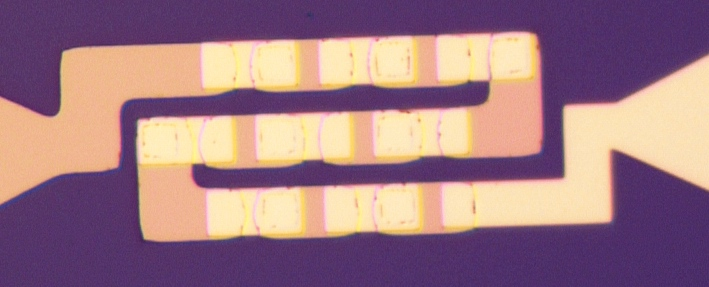
\includegraphics[width=0.5\paperwidth]{img/04/fab_series_9_zoom.jpg}
        \caption{Przykładowa struktura połączeń wykorzystywana w czasie eksperymentu.}
        \label{FabricationSubstrate}
    \end{figure}
	
	Później opisano metody pomiarowe stosowane do charakteryzacji komórek pamięci STT-MRAM oraz przedstawiono rezultaty pomiarów. Jako efekt końcowy osiągnięto funkcjonalną 3-bitową strukturę pamiętającą.


    \begin{figure}[H]
        \centering
        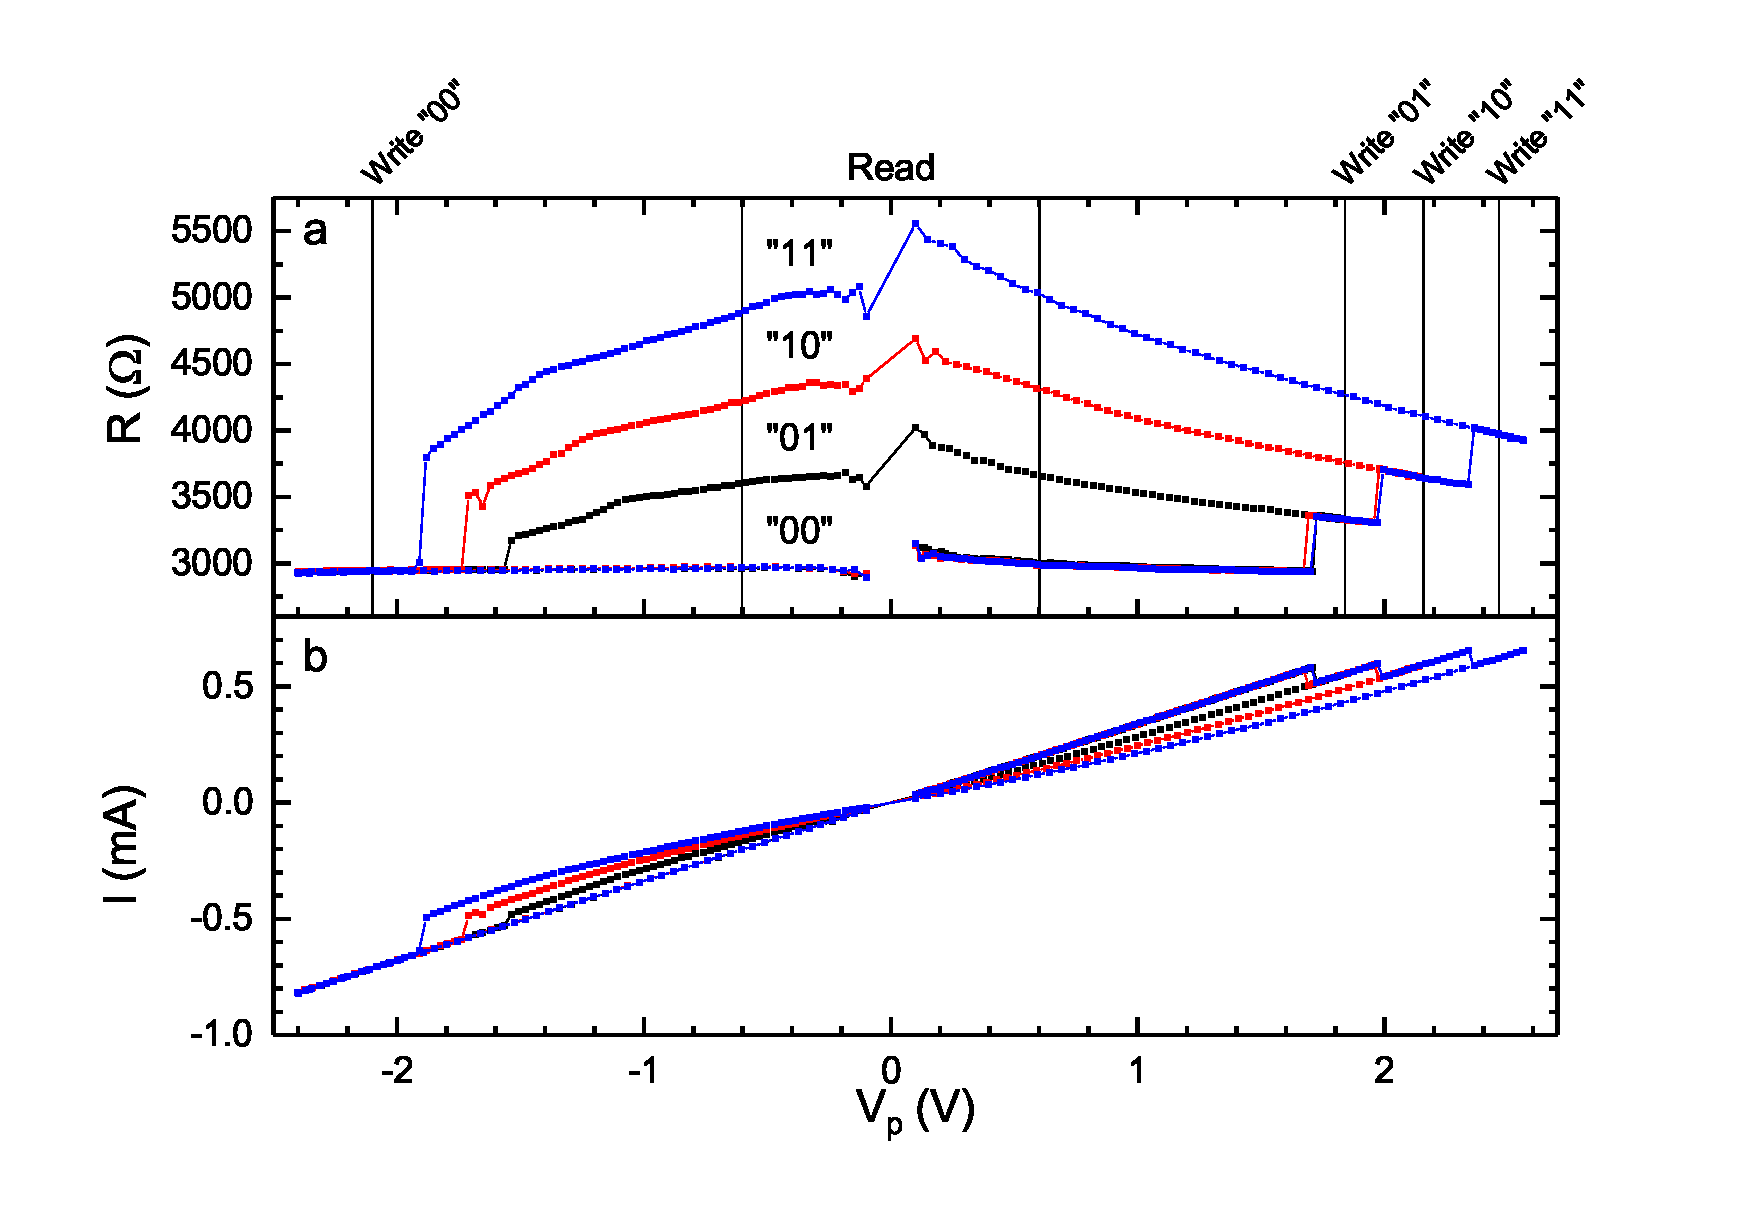
\includegraphics[width=0.5\paperwidth]{img/05/ResultsCIMS2.eps}
        \caption{Rezultaty pomiaru CIMS dla 2-bitowej struktury pamiętającej. Zaproponowano kodowanie binarne, napięcia do zapisu i region bezpieczny dla odczytu (a). Zmiany prądu w czasie pomiarów (b).}
        \label{ExperimentMeasurementCIMS2}
    \end{figure}

    \begin{figure}[H]
        \centering
        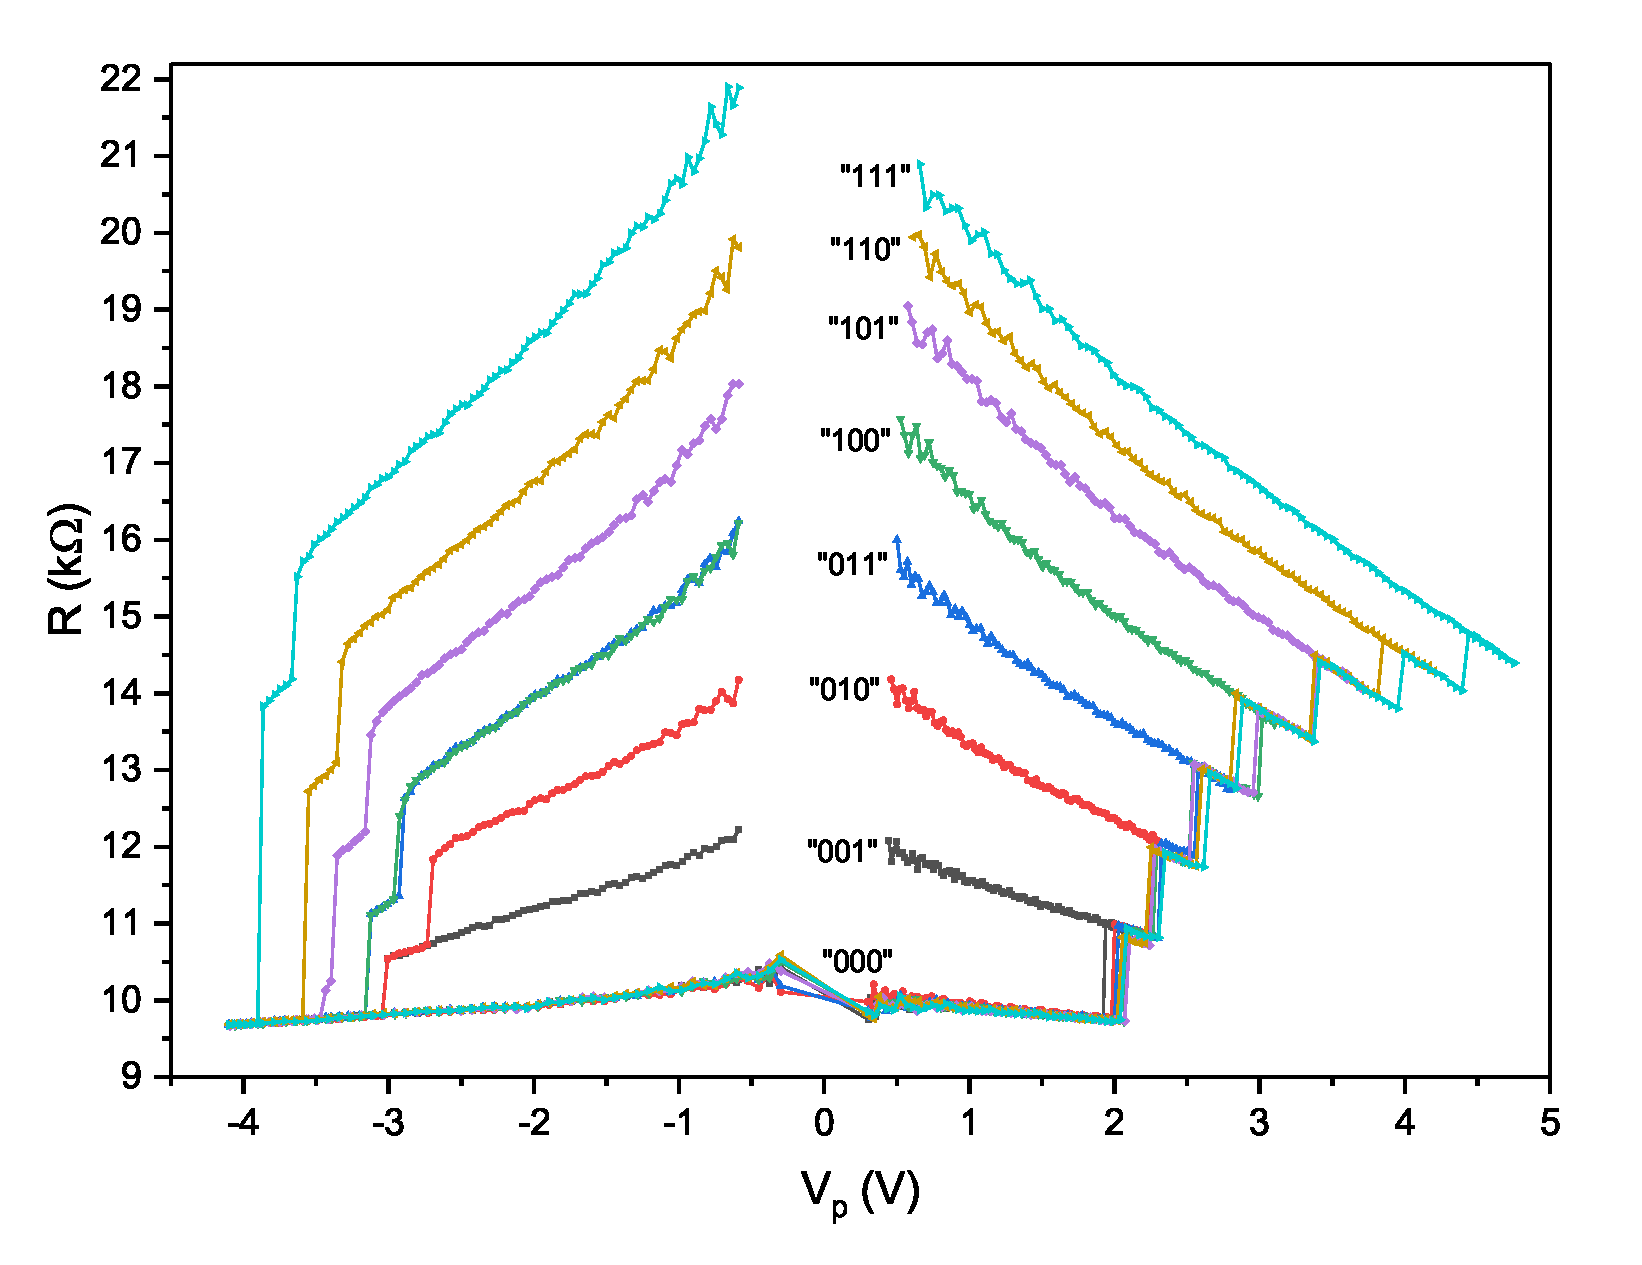
\includegraphics[width=0.5\paperwidth]{img/05/ResultsCIMS3.eps}
        \caption{Rezultaty pomiaru CIMS dla 3-bitowej struktury pamiętającej. Zaproponowano kodowanie binarne.}
        \label{ExperimentMeasurementCIMS3}
    \end{figure}

    
    W podsumowaniu omówiono wszystkie osiągnięte rezultaty a także zwrócono uwagę na niedoskonałości proponowanego rozwiązania i zaproponowano dalszy kierunek badan i optymalizacji.
%\include{04_fabricationPL}
%\include{05_experimentPL}

%\chapter{Acknowledgements}

	This work is supported by the Polish Ministry of Science and Higher Education \textbf{Diamond Grant No. 0048/DIA/2017/46} and the Polish National Center for Research and Development grant No. \textbf{LIDER/467/L-6/14/NCBR/2015}.
	
    \vspace{2cm}
    
    I would like to express my profound gratitude to \textbf{my parents}, for their support and invaluable help at every moment of my life.

    I would like to thank my supervisor, \textbf{PhD Witold Skowroński}, for his help in preparing the work and carrying out the experiments.

	I am very grateful to \textbf{Professor Tomasz Stobiecki}, for giving me an opportunity to explore the world of science.

    I would like to thank \textbf{PhD Sławomir Ziętek}, for his help in carrying out the experiments.
    
    I am grateful to \textbf{Academic Center of Materials and Nanotechnology (ACMiN AGH)} and \textbf{Professor Marek Przybylski} for an opportunity to perform nanostructurization of the sample. I would also like to thank \textbf{Singulus AG} and \textbf{PhD Jerzy Wrona} for providing the sample with MTJ stack deposited.





%\appendix
%\printbibliography

\end{document}
